\subsection{Anreise}

Anreise


\begin{figure}[H]
	\centering
	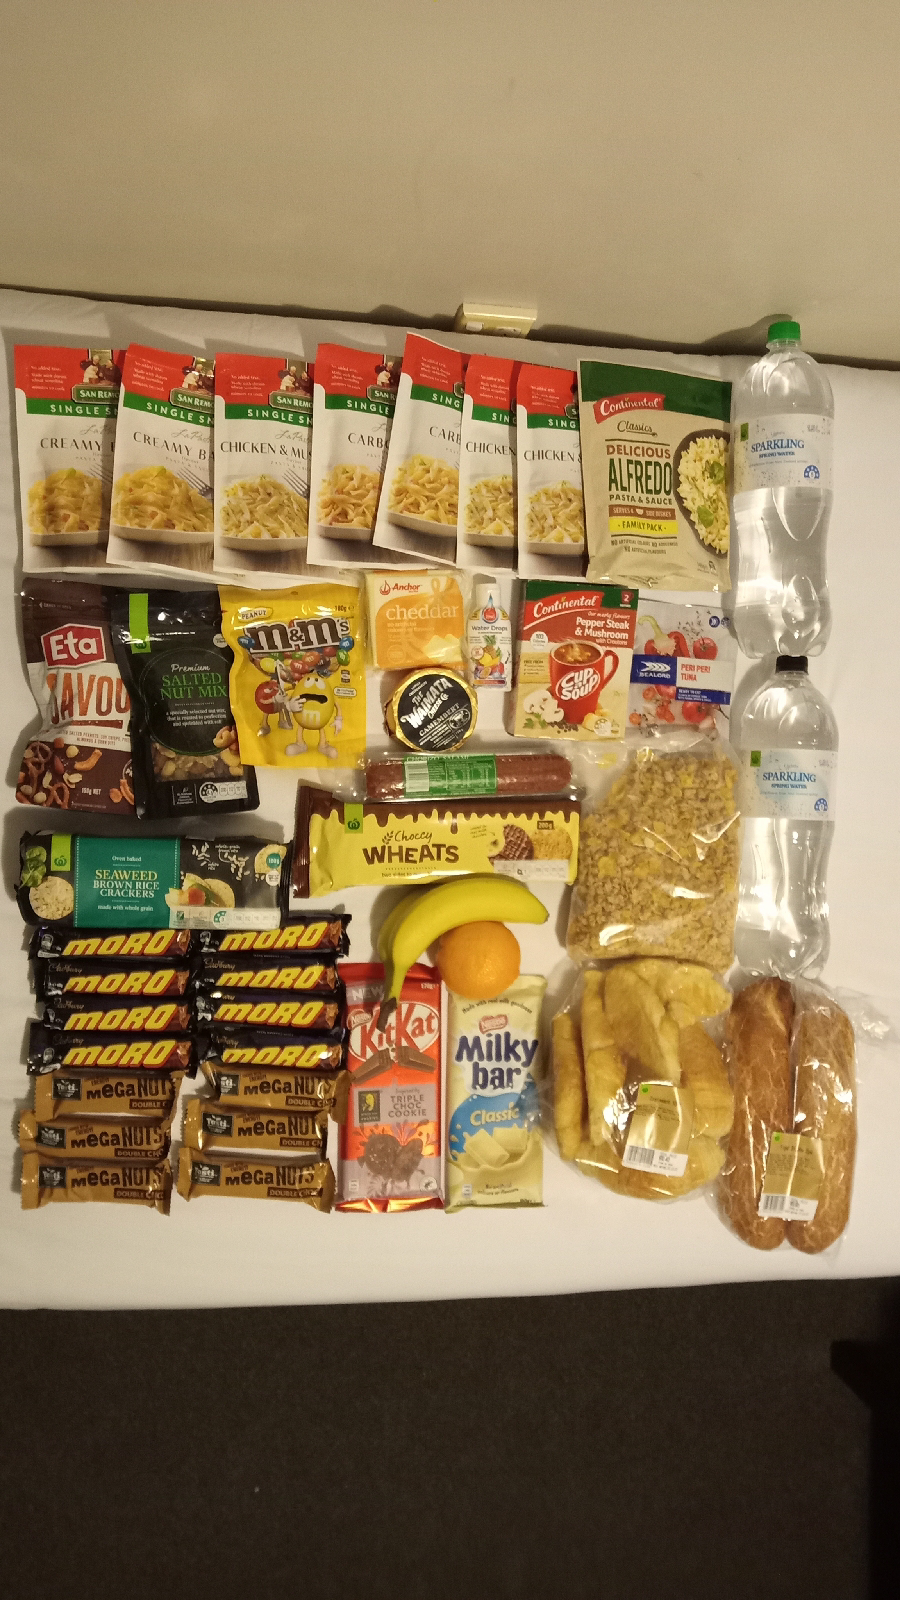
\includegraphics[width=0.5\textwidth]{anreise/5_1665920991125980-0.png}
	\caption{}
	\label{fig:5_1665920991125980-0}
\end{figure}

  Am Donnerstag den 14.10.22 starten wir unser Neuseeland Abenteuer 22/23.
 


  Nach einer recht langen Anreise mit Bahn, Bus und etlichen Flugzeugen haben wir heute gegen 12:00 Uhr, unseren ersten Zielort in Kerikeri erreicht.
 


  Zunächst ging es mit der Bahn von Grafing Bhf mit Umsteigen in München, Stuttgart und Mannheim nach Basel.
 


\begin{figure}[H]
	\centering
	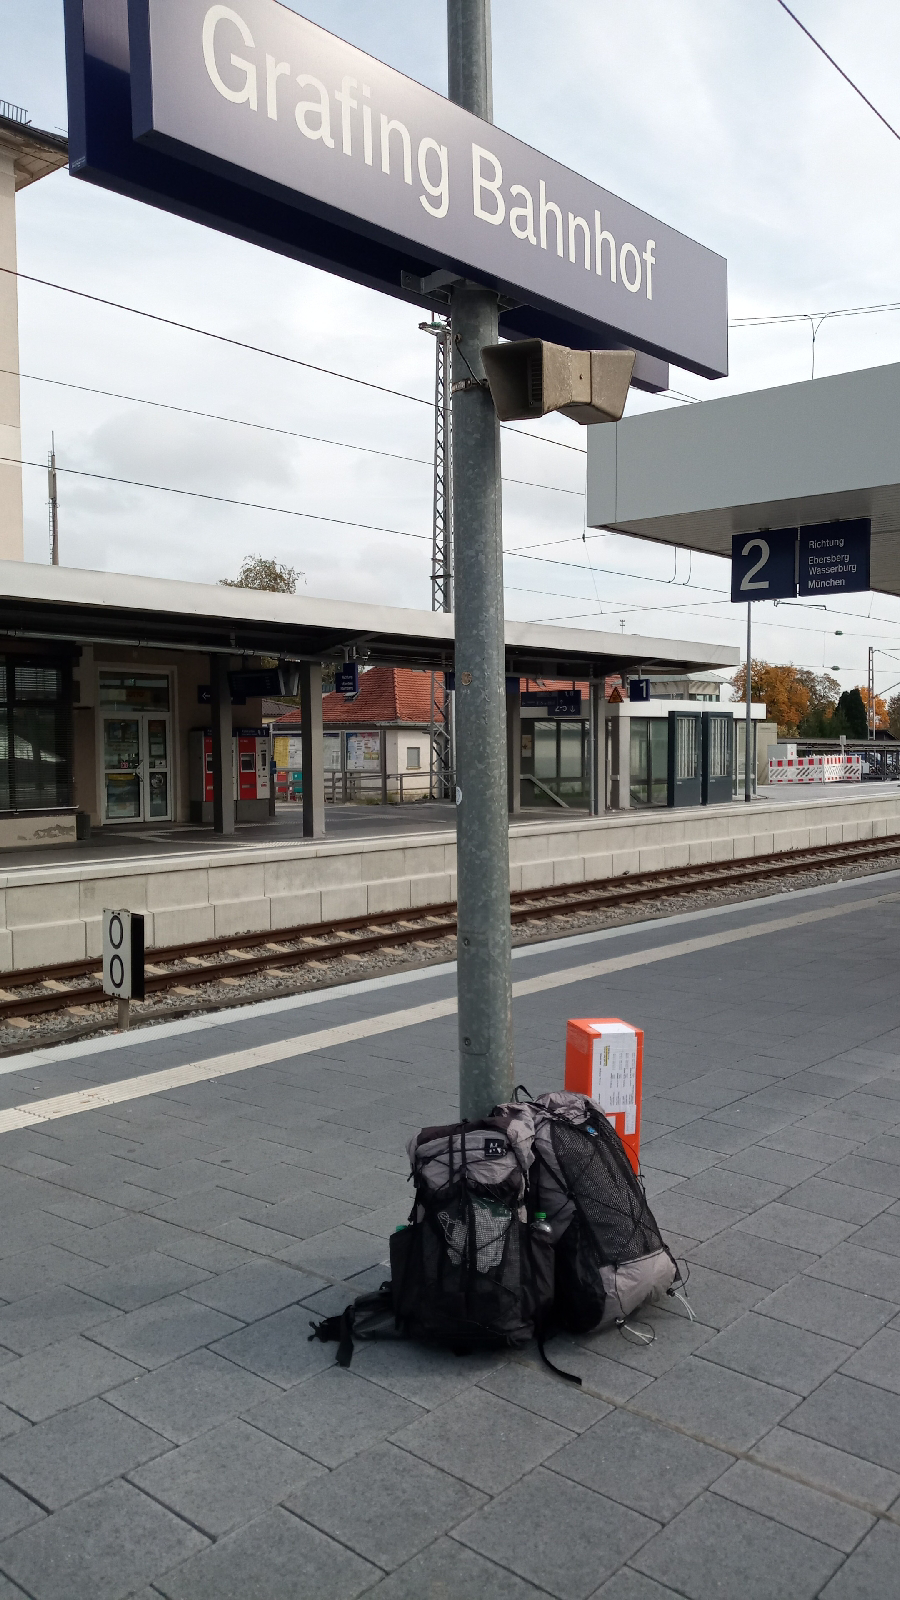
\includegraphics[width=0.5\textwidth]{anreise/6_1665920645823194-0.png}
	\caption{}
	\label{fig:6_1665920645823194-0}
\end{figure}

  Nach einer Nacht, in einem Hotel direkt neben dem Airport Basel,  folgten etliche kurze und längere Flüge. Zunächst nach Frankfurt, von dort nach Seoul in Südkorea (11:30 Flugzeit).
 


\begin{figure}[H]
	\centering
	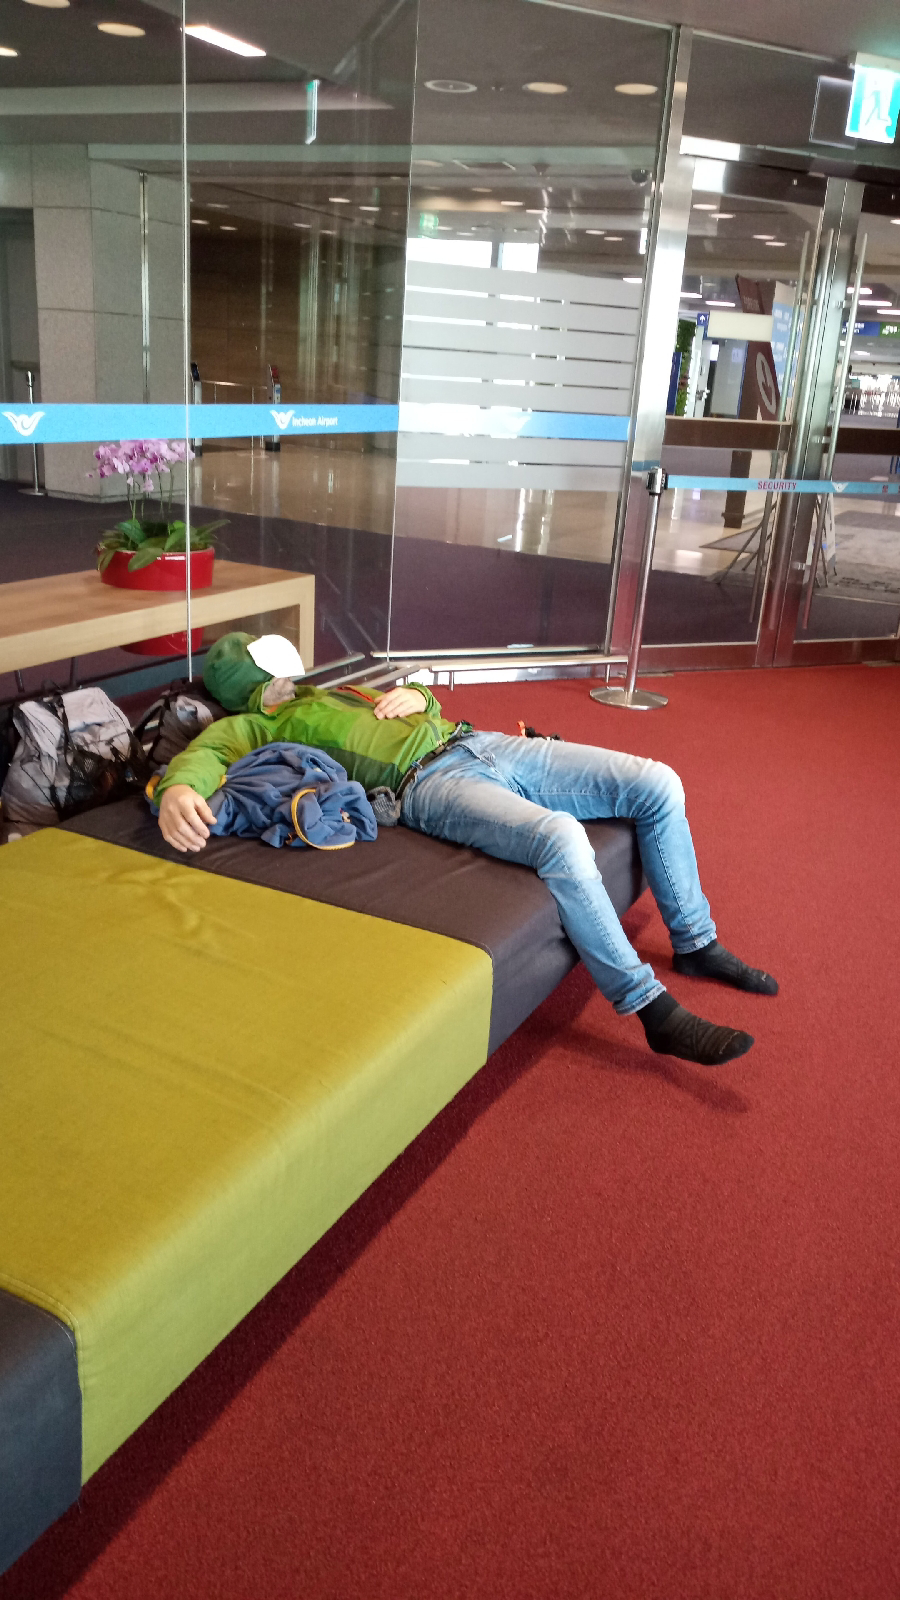
\includegraphics[width=0.5\textwidth]{anreise/7_1665920641399421-1.png}
	\caption{}
	\label{fig:7_1665920641399421-1}
\end{figure}

  Nach ein paar Stunden Aufenthalt folgte der Weiterflug nach Auckland (11:30 Flugzeit). Die dortige Einreise verlief problemlos, alle Dokumente waren in Ordnung auch der kleine Bio Security Hund hatte keine Lust auf uns. Zum Thema Corona gab es sowohl hier, als auch bei den anderen Stops keine Nachfragen. Wir hoffen die  nächsten Monate von diesem Thema verschont zu bleiben.
 


  Den letzten Flug Richtung Norden, nach Kerikeri, konnten wir kostenlos umbuchen (typisch Neuseeland) und schon einen Flieger früher besteigen.
 


\begin{figure}[H]
	\centering
	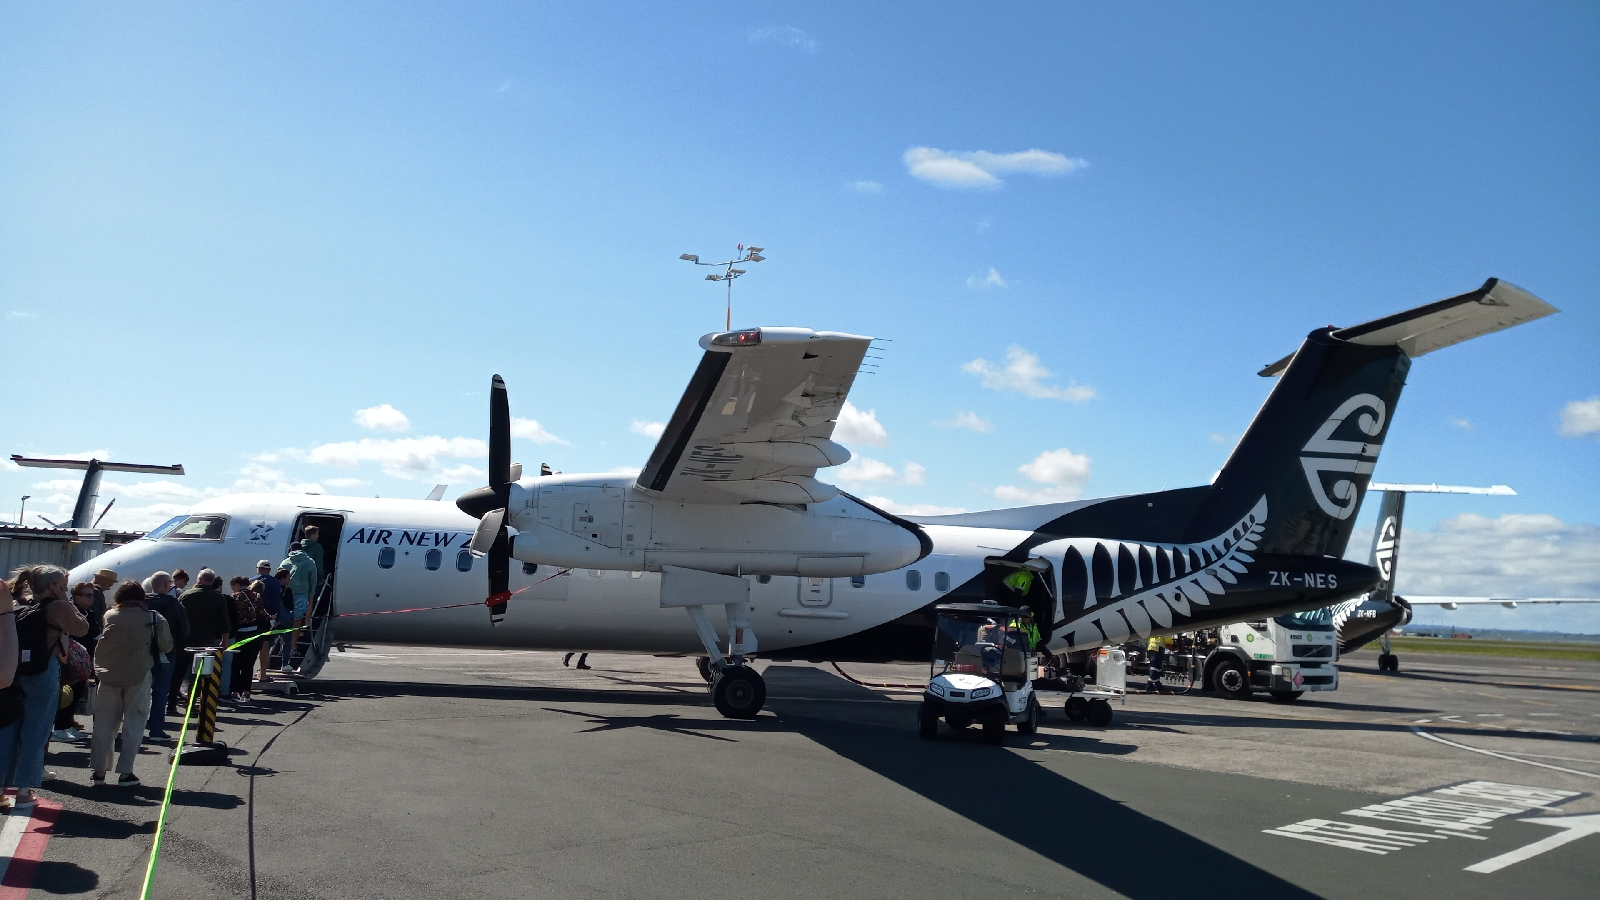
\includegraphics[width=0.5\textwidth]{anreise/8_1665920636856896-2.png}
	\caption{}
	\label{fig:8_1665920636856896-2}
\end{figure}

\begin{figure}[H]
	\centering
	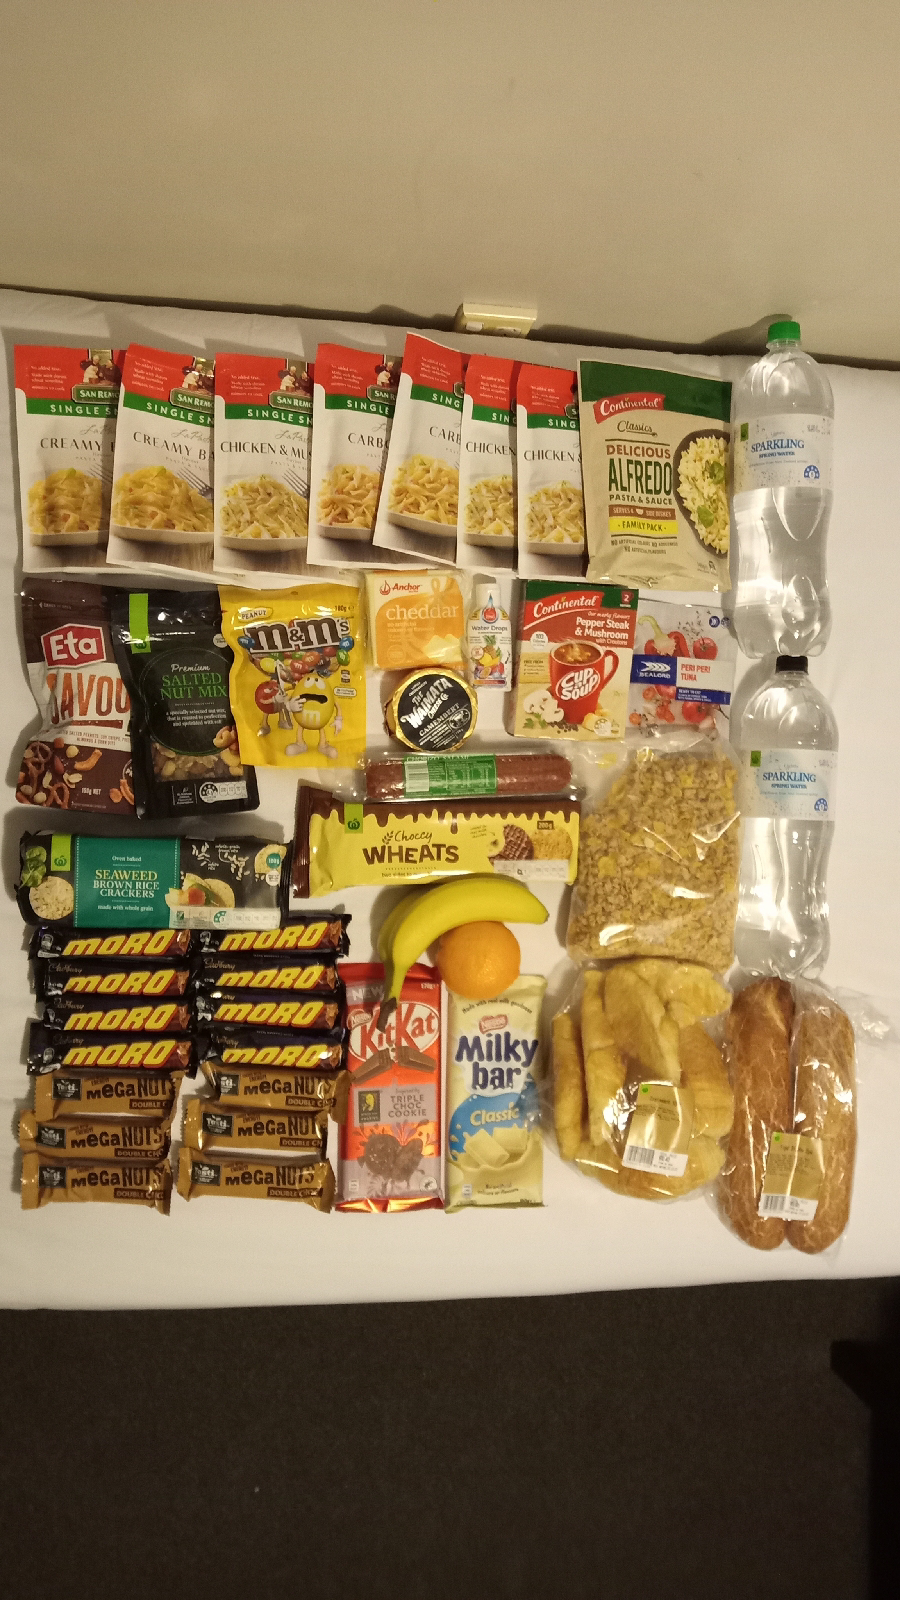
\includegraphics[width=0.5\textwidth]{anreise/9_1665920631783425-3.png}
	\caption{}
	\label{fig:9_1665920631783425-3}
\end{figure}

  Zusätzlich mussten wir noch eine Sim Karte für Neuseeland besorgen, mit der ich leider noch nicht telefonieren kann aber immerhin schon das Internet zur Verfügung steht. Dank Niklas's Tipp war auch der Kauf der Gasflasche bei Hunting and Fishing gleich erledigt.
 


  So, morgen hoffen wir bis zur  Nordspitze zu kommen, das sind nur etwa 175 km, müsste doch per Anhalter auch ohne Mitfahrerbankerl zu schaffen sein. Es ist jetzt kurz nach Mitternacht, Petra schläft schon einige Zeit und ich brauche jetzt auch etwas Ruhe. Bis Bald und viele liebe Grüße nach Hause, besonders an diejenigen, denen es zur Zeit vielleicht nicht so gut geht.
 

